\clearpage
\section{QUESTÕES DE DESENVOLVIMENTO}
\label{section}
\subsection{Representação da situação por meio de um grafo}
Consideremos o grafo abaixo apresentado como G:\\
\begin{figure}[h]
    \centering
    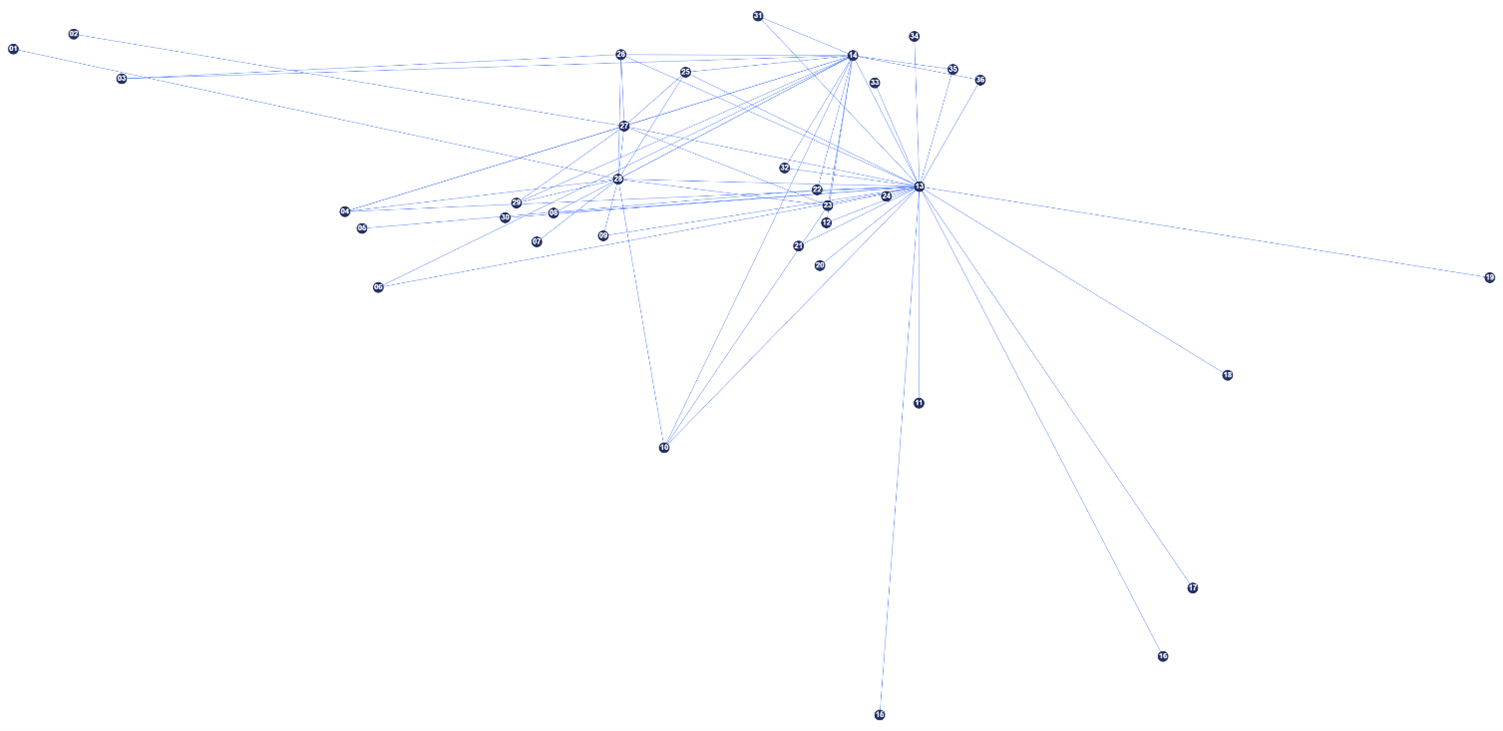
\includegraphics[width=0.8\textwidth]{imgs/Figura11}
    \caption{Grafo G\label{fig:imagem11}}
\end{figure}
\subsection{ O grafo é conexo?}
\indent Por definição, um grafo é conexo quando é possível ligar quaisquer dois vértices pertencentes a esse grafo, por meio de uma cadeia. O grafo representado na Figura 10 é conexo.\\
\indent No grafo G, na Figura 11, escolhendo quaisquer dois vértices, existem ligações entre si por uma aresta ou por um conjunto de arestas que passam por outros vértices intermédios numa cadeia.\\
\indent Em contexto com o objetivo deste trabalho, podemos dizer que o mapa de rotas aéreas representam um 
grafo conexo.\\
\indent Um exemplo em concreto disso é a ligação entre Londres, na Inglaterra, e Phuket, na Tailândia. Neste 
caso não existe uma ligação direta entre estas cidades, mas é possível ir de uma para a outra, fazendo escala 
por Aktau, e depois por Almaty. Esta situação existe para quaisquer dois destinos à nossa escolha por onde a 
Air Astana opera. Bem, não necessariamente fazendo escala pelos destinos referidos, mas sim por outros.\\
\subsection{O grafo é euleriano?}
\indent Leonhard Paul Euler, o matemático e físico suíço que resolveu o problema conhecido como as sete pontes de Königsberg. 
Determinados grafos são categorizados como grafos eulerianos, satisfazendo certas condições
e propriedades traduzidas por Euler, e daí os certos grafos terem o seu nome.\\
\indent Para um grafo se designar como euleriano, tem de ser possível partir de um determinado vértice,
percorrer todas as arestas de um grafo sem as repetir e terminar no vértice de partida. Portanto, um grafo 
euleriano é uma cadeia simples fechada, um ciclo euleriano. De notar que é possível ter uma cadeia euleriana, 
sendo que a principal diferença está no ponto de partida e no de chegada, serem diferentes.\\
\indent O grafo G, da figura 11, é euleriano? Tem um ciclo euleriano? Observando o grafo a resposta é simples, 
não se trata de um grafo euleriano. Um dos exemplos disso é olhar para o vértice 01 e ver que possui apenas 
uma aresta adjacente. É possível partir de 01 pela sua aresta adjacente, mas para regressar a 01 usando essa 
mesma aresta, já não se aplica a definição de ciclo euleriano. G também não é uma cadeia euleriana, pois
observando novamente o grafo, existem vários destinos com apenas uma aresta adjacente, e para percorrer 
todos os vértices, seria preciso repetir essas arestas no percurso da cadeia.\\
\\
\indent Euler estabeleceu dois Teoremas para a determinação de grafos euleriano:\\
\\
\begin{itemize}
\item 
\verb|Teorema 1| um dado grafo, conexo, tem uma cadeia euleriana se e só se o número de vértices de grau ímpar, ser dois, nesse grafo.
\item 
\verb|Teorema 2| um dado grafo, conexo, tem um ciclo euleriano se e só se todos os seus vértices têm grau par.
\end{itemize}
\indent Graficamente verificou-se que G não se trata nem de uma cadeia nem de um ciclo euleriano. Vejamos 
agora por meio dos teoremas. Para isso, temos de determinar o grau de todos os vértices de G, relembrando 
que \underline{deg(v) = nº de arestas adjacentes a v.} \\

\begin{center}
    \begin{tabular}{ |c|c|c|c|c|c| } 
     \hline
     deg(01)= 1 & deg(07)= 1 & deg(13)= 29 & deg(19)= 1 & deg(25)= 4 & deg(31)= 2\\
     \hline
     deg(02)= 1 & deg(08)= 2 & deg(14)= 18 & deg(20)= 1 & deg(26)= 5 & deg(32)= 2\\
     \hline
     deg(03)= 2 & deg(09)= 2 & deg(15)= 1 & deg(21)= 1 & deg(27)= 9 & deg(33)= 1\\
     \hline
     deg(04)= 4 & deg(10)= 4 & deg(16)= 1 & deg(22)= 3 & deg(28)= 12 & deg(34)= 1\\
     \hline
     deg(05)= 1 & deg(11)= 1 & deg(17)= 1 & deg(23)= 5 & deg(29)= 3 & deg(35)= 2\\
     \hline
     deg(06)= 2 & deg(12)= 2 & deg(18)= 1 & deg(24)= 1 & deg(30)= 1 & deg(36)= 2\\ 
     \hline
     $\sum_{}^{}deg(v)=$130 &   &   &   &   & \\
     \hline
    \end{tabular}
\end{center}

\indent Por meio da tabela acima, vemos que o número de vértices de grau ímpar, ultrapassa facilmente o dois, e 
daí concluímos que não existe uma cadeia euleriana. Como os vértices não são todos de grau par, não existe 
um ciclo euleriano.\\
\\
\indent Vamos interpretar agora, no contexto do problema, que se considerássemos todas as rotas aqui 
representadas da companhia aérea, em que cada uma duplicar-se-ia em trajetos distintos, um de ida e outra
de volta, nós teríamos um grafo euleriano no mapa.
Vejamos o exemplo na figura seguinte, entre Almaty (13) e Seoul (19):\\
\begin{figure}[h]
    \centering
    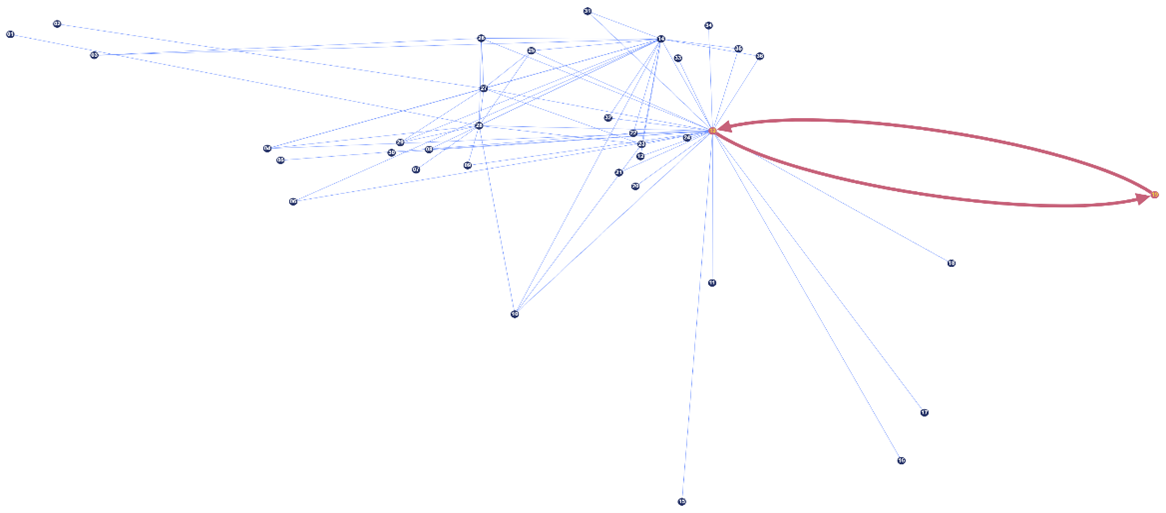
\includegraphics[width=0.8\textwidth]{imgs/Figura12}
    \caption{Exemplo de digrafo associado\label{fig:imagem12}}
\end{figure}
\indent Damos o exemplo entre os dois destinos salientados, na figura 12, como arestas orientadas. Caso 
aplicássemos o mesmo em todas as arestas de G, passaríamos a ter um digrafo associado ao grafo G. Desta 
forma o agora digrafo já se classificaria como euleriano, pois o grau de todos os vértices passaria a ser par.
Daqui, comprovar-se-ia outro teorema para digrafos, onde $\tau^+(v)$=$\tau^-(v)$
para cada vértice v, o que admite, um circuito euleriano.\\
   
\subsection{ O grafo é hamiltoniano? }
William Rowan Hamilton, matemático, físico e astrónomo irlandês. Terá sido a partir do jogo do icosaedro
que se deu a origem do grafo hamiltoniano. As condições para se verificar um grafo hamiltoniano, implicam
que se faça uma cadeia, ou caminho, por todos os vértices sem se repetir nenhum.\par
Existem cadeias e ciclos hamiltonianos para grafos. No caso de digrafos, existem caminhos e circuitos 
hamiltonianos.\par
Nos dias de hoje ainda não é possível encontrar um método sucinto e simples, que satisfaçam as
condições de grafo hamiltoniano, como acontece no caso dos grafos eulerianos. A solução passa por seguir 
regras que mais satisfazem a condição oposta, ou seja, ajudam a verificar se os grafos em estudo não são 
hamiltonianos.\par
Interpretando agora o grafo G que representa as rotas da Air Astana. Se tentarmos desenhar um ciclo 
onde começamos pelo vértice 01 (Londres), temos logo obrigatoriamente que passar pelo vértice 28 (Aktau). 
Para completar o ciclo terminando em Londres, teríamos de repetir o vértice 28. É uma das muitas situações 
bem visíveis graficamente, o que nos leva a concluir que não se trata de um grafo hamiltoniano.\par
As regras para tentativa de construção de um ciclo hamiltoniano são:\par
\begin{itemize}
    \item \verb|Regra 1| - Se um vértice v tem grau 2, então ambas as arestas incidentes nesse vértice devem fazer parte 
    do ciclo hamiltoniano;\\
    \item  \verb|Regra 2| -  Durante a construção de um ciclo hamiltoniano, nenhum ciclo deve ser formado até todos os 
    vértices terem sido visitados;\\
    \item \verb|Regra 3| - Se durante a construção de um ciclo hamiltoniano duas das arestas incidentes ao vértice v estão 
    no ciclo, então todas as outras arestas incidentes nesse vértice podem ser apagadas (não podem entrar no 
    ciclo).\\
\end{itemize}
Vamos observar no grafo os vértices 06, 13, 14 e 36:\par
%inserir figura 13
Obrigatoriamente os vértices 06 e 36, pela regra 1, por cada um deles ser de grau 2, as suas arestas fazem 
parte do ciclo hamiltoniano. Acontece que ambos ficam ligados aos vértices 13 e 14, implica logo que a regra 3 
seja aplicada a estes últimos vértices. Como estes já possuem duas arestas pertencentes ao ciclo, teríamos de 
descartar todas as outras adjacentes aos mesmos, o que na prática excluía imensos vértices do grafo, por 
possuírem grau 1. Conclusão, o grafo é não é hamiltoniano.\par
Outro ponto de vista assenta pelo não cumprimento da regra 2. Ao aplicar a regra 1 aos vértices 06 e 36 
por obrigatoriedade, e como consequência também da regra 3 aos vértices 13 e 14, forma-se um ciclo entre 
estes 4 vértices, ignorando todos os outros. Logo, o grafo não é hamiltoniano.\par
\subsection{ Matriz de adjacência do grafo G }
Uma matriz de adjacência traduz-se por uma tabela de dupla entrada onde se lista o número de ligações 
entre dois dados vértices.\par
%inserir tabela 2
\textbf{Observação:} Como o grafo apresentado é um grafo simples, o que implica que não existem mais do que 
uma aresta igual entre dois vértices ligados, esta matriz de adjacência coincide com uma matriz Booleana.\par
Uma matriz booleana ignora o número de arestas iguais existentes entre dois vértices como por exemplo 
no caso dos multigrafos, focando-se apenas se existe ligação ou não entre dois vértices. Existindo ligação, na 
matriz representa-se com 1, não existindo representa-se com 0.\par

\subsection{  Fecho transitivo direto de um vértice }
O fecho transitivo direto de um vértice qualquer v, é um conjunto de vértices que é possível chegar a
partir de v, por meio de uma cadeia ou caminho, com um comprimento qualquer. Usa-se uma matriz booleana 
para o efeito, e normalmente usa-se uma coluna auxiliar à direita da matriz booleana para facilitar a 
demonstração do fecho.\par
Começamos por escolher um vértice qualquer v, vamos escolher o 01, como ponto de partida. Na coluna
auxiliar, na posição do vértice 01, coloca-se um zero, pois para ir do vértice ao próprio vértice, é preciso uma 
cadeia de comprimento zero. Faz-se depois uma passagem pela matriz booleana na linha da posição do vértice
01, e aponta-se todos os vértices com ligação a 01. Só existe o 28 na linha do 01. Transcreve-se na posição 28
da coluna auxiliar, com incremento do nível seguinte, neste caso 1. Significa que para chegar de 01 a 28 é 
preciso uma cadeia ou caminho de comprimento 1. Passamos agora pela linha do vértice 28 para verificar
todos os vértices ligados a 28 e anota-se na coluna auxiliar todos os vértices ligados, nas suas respetivas 
posições, ficando neste caso, novo incremento do nível seguinte (2) nas posições dos vértices 29, 27, 26, 25, 
23, 14, 13, 10, 09, 07, 04, e supostamente no 01 também. Mas aqui a particularidade é que já existe ligação 
com nível menor no 01, logo não alteramos nada em 01.\par
Na matriz deste grafo aqui representada, acabamos por ter um esquema deste género, para os 3 
primeiros vértices:\par
%inserir figura 14
Temos de fazer algumas observações. O vértice 28 tem nível 1, os vértices 29, 27, 26, 25, 23, 14, 13, 10, 
09, 07, 04 tem todos nível 2, a partir daqui temos de atribuir o nível 3 a todos os vértices que ligam aos de 
nível 2.\par
Outra observação a ter em conta é que o fecho transitivo lista o comprimento mínimo necessário para se 
chegar de um vértice. Podemos ter, em alguns casos cadeias ou caminhos de comprimento infinito, repetindo 
arestas.\par
O fecho transitivo direto de um vértice é representado por $\Gamma$v e é um conjunto. No caso do vértice 01, 02 e 
03 temos:\par
$\Gamma$1 =\\
\{01,02,03,04,05,06,07,08,09,10,11,12,13,14,15,16,17,18,19,20,21,22,23,24,25,26,27,28,
29,30,31,32,33,34,35,36\};\par
$\Gamma$ 2 =\\
\{01,02,03,04,05,06,07,08,09,10,11,12,13,14,15,16,17,18,19,20,21,22,23,24,25,26,27,28,
29,30,31,32,33,34,35,36\};\par
$\Gamma$ 3 =\\
\{01,02,03,04,05,06,07,08,09,10,11,12,13,14,15,16,17,18,19,20,21,22,23,24,25,26,27,28,
29,30,31,32,33,34,35,36\}.\par
\subsection{ Fecho transitivo inverso de um vértice }
O fecho transitivo inverso de um vértice v, retrata o oposto ao fecho transitivo direto. É um conjunto de 
vértices que a partir desses mesmos é possível chegar a v.\par
O método de determinação do fecho inverso é semelhante ao de fecho transitivo direto, com a diferença 
que usamos linhas auxiliares abaixo da matriz booleana ao invés de colunas. Para determinar as ligações dos 
vértices na própria matriz, percorremos as colunas dos vértices em questão ao invés das linhas. De resto, todas as 
regras e observações já listadas na questão anterior aplicam-se também ao fecho transitivo inverso. Representa-se por $\Gamma^{-1}$ v e é um conjunto.\par 
Segue agora a disposição da matriz com os fechos transitivos inversos dos 3 primeiros vértices, representados abaixo da matriz booleana:\par
%inserir figura 15
$\Gamma^{-1}$1 =\\
\{01,02,03,04,05,06,07,08,09,10,11,12,13,14,15,16,17,18,19,20,21,22,23,24,25,26,27,28,
29,30,31,32,33,34,35,36\};\par
$\Gamma^{-1}$ 2 =\\
\{01,02,03,04,05,06,07,08,09,10,11,12,13,14,15,16,17,18,19,20,21,22,23,24,25,26,27,28,
29,30,31,32,33,34,35,36\};\par
$\Gamma^{-1}$ 3 =\\
\{01,02,03,04,05,06,07,08,09,10,11,12,13,14,15,16,17,18,19,20,21,22,23,24,25,26,27,28,
29,30,31,32,33,34,35,36\}.\par
%adicionar chavetas

\subsection{ Relação entre os fechos transitivos diretos e inversos }
Podemos retirar conclusões adicionais sobre a matriz booleana e os fechos de um vértice. A partir da 
matriz booleana do grafo em questão podemos ver que a soma de cada linha da matriz, ou cada coluna dá-nos o 
grau do vértice associado.\par
A reunião do fecho transitivo direto com o fecho transitivo inverso de qualquer vértice deste grafo, 
dá-nos o conjunto de todos os vértices do grafo, logo, o grafo é conexo, reforçando o que já foi dito acima.\par